% +------------------------------------------------------------------------+
% | Reference manual page: Tds_3.tex
% +------------------------------------------------------------------------+
% | 27.3.2000   Monique Teillaud
% | Package: Triangulation3
% | 
\RCSdef{\RCSTdsRev}{$Revision$}
\RCSdefDate{\RCSTdsDate}{$Date$}
% |
%%RefPage: end of header, begin of main body
% +------------------------------------------------------------------------+


\begin{ccRefConcept}{TriangulationDataStructure_3}

%% \ccHtmlCrossLink{}     %% add further rules for cross referencing links
%% \ccHtmlIndexC[concept]{} %% add further index entries

\ccDefinition

3D-triangulation data structures are meant to maintain the
combinatorial information for 3D-geometric triangulations.

In \cgal, a triangulation data structure is a
container of cells ($3$-faces) and vertices ($0$-faces). Each cell gives
access to its four incident vertices and to its four adjacent
cells. Each vertex gives direct access to one of its incident cells, which is 
sufficient to retrieve all the incident cells when needed.

The four vertices of a cell are indexed with 0, 1, 2 and 3.  The
neighbors of a cell are also indexed with 0, 1, 2, 3 
in such a way that the neighbor indexed by $i$ is opposite to the vertex
with the same index (see Figure~\ref{TDS3-fig-repres}).

Edges ($1$-faces) and facets ($2$-faces) are not explicitly
represented: a facet is given by a cell and an index (the facet
\ccc{i} of a cell \ccc{c} is the facet of \ccc{c} that is opposite to
the vertex of index \ccc{i}) and an edge is given by a cell and two
indices (the edge \ccc{(i,j)} of a cell \ccc{c} is the edge
whose endpoints are the vertices of indices \ccc{i} and \ccc{j} of
\ccc{c}). 

As \cgal\ explicitly deals with all degenerate cases, a
3D-triangulation data structure in \cgal\ can handle the cases when
the dimension of the triangulation is lower than~3 
(see Section~\ref{TDS3-sec-intro}).

Thus, a 3D-triangulation data structure can store a triangulation of a
topological sphere $S^d$ of $\R^{d+1}$, for any $d \in \{-1,0,1,2,3\}$. 

\bigskip

The second template parameter of the basic triangulation class 
(see Chapter~\ref{chapter-Triangulation3})
\ccc{Triangulation_3<TriangulationTraits_3,TriangulationDataStructure_3>} is a triangulation 
data structure class. (See Chapter~\ref{chapter-TDS3}.)  

To ensure all the \textbf{flexibility} of class \ccc{Triangulation_3}
described in 
\lcTex{ \ccRefPage{CGAL::Triangulation_3<TriangulationTraits_3,TriangulationDataStructure_3>}
and in } Chapter~\ref{chapter-Triangulation3}, a model of a
triangulation data structure must be templated by the base vertex and
the base cell classes (see~\ref{TDS3-sec-intro}):
\ccc{TriangulationDataStructure_3<TriangulationVertexBase_3,TriangulationCellBase_3>}.
The optional functionalities related to geometry are compulsory for
this use as a template parameter of \ccc{Triangulation_3}.

\bigskip

A class that satisfies the requirements for a
triangulation data structure class must provide the following types and
operations. 

\ccTypes
\ccThree{typedef triple <Cell*, int, int>}{Facet }{}
\ccThreeToTwo

\ccNestedType{Vertex }{}
\ccGlue
\ccNestedType{Cell}{Cell type}
\lcTex{
Requirements for \ccc{Vertex} and \ccc{Cell} are described in
\ccRefPage{TriangulationDataStructure_3::Vertex} and \ccRefPage{TriangulationDataStructure_3::Cell}.
}

\ccTypedef{typedef triple<Cell*, int, int> Edge;}{\ccc{(c,i,j)} is the
edge of cell \ccc{c} whose vertices indices are \ccc{i} and
\ccc{j}. (See Section~\ref{TDS3-sec-intro}.)}
\ccGlue
\ccTypedef{typedef pair<Cell*, int>  Facet;}{\ccc{(c,i)} is the facet
of \ccc{c} opposite to the vertex of index \ccc{i}. (See
Section~\ref{TDS3-sec-intro}.)} 


The following iterators allow one to visit all the vertices, edges, facets
and cells of the triangulation data structure. They are all
bidirectional, non-mutable iterators.

\ccNestedType{Cell_iterator}{}
\ccGlue
\ccNestedType{Facet_iterator}{}
\ccGlue
\ccNestedType{Edge_iterator}{}
\ccGlue
\ccNestedType{Vertex_iterator}{}

The following circulators allow us to visit all the cells and facets
incident to a given edge. They are bidirectional and non-mutable.

\ccNestedType{Facet_circulator}{}
\ccGlue
\ccNestedType{Cell_circulator}{}

\ccCreation
\ccCreationVariable{tds}  %% choose variable name
\ccThree{TriangulationDataStructure_3<Tvb,Tcb>();}{tds.set_number}{}
\ccThreeToTwo

\ccConstructor{TriangulationDataStructure_3();}
{A default constructor.}

\ccConstructor{TriangulationDataStructure_3(const TriangulationDataStructure_3 & tds1);}
{Copy constructor. All the vertices and cells are duplicated.}

\ccMethod{TriangulationDataStructure_3 operator = (const TriangulationDataStructure_3 & tds1);}
{Assignment. All the vertices and cells are duplicated.}

The previous two methods are equivalent.

\ccThree{Vertex*xx}{tds.insert_in_facet()}{}

\ccMethod{void swap(TriangulationDataStructure_3 & tds1);} 
{Swaps \ccVar\ and \ccc{tds1}. There is no copy of cells and vertices,
thus this method runs in constant time. This method should be preferred to
\ccVar=\ccc{tds1} or \ccVar(\ccc{tds1}) when \ccc{tds1} is deleted after
that.}

\ccMethod{Vertex* copy_tds(const TriangulationDataStructure_3 & tds1, Vertex* v = NULL);}
{\ccc{tds1} is copied into \ccVar. If $v\, !\!= NULL$, the vertex of \ccVar\ 
corresponding to \ccc{v} is returned, otherwise \ccc{NULL} is returned.
\ccPrecond{The optional argument \ccc{v} is a vertex of \ccc{tds1}.}}

\ccFunction{void ~tds();}
{Destructor. All vertices and cells are deleted, and \ccVar\ itself is
deleted.} 

\ccOperations

\ccAccessFunctions

\ccMethod{int dimension() const;}
{The dimension of the triangulated topological sphere.}

\ccMethod{int number_of_vertices() const;}
{The number of vertices. Note that the triangulation data structure has one
more vertex than an associated geometric triangulation, if there is
one, since the infinite vertex is a standard vertex and is thus also
counted.} 

\ccHeading{Non constant-time access functions}
\ccMethod{int number_of_cells() const;}
{The number of cells. Returns 0 if \ccVar.\ccc{dimension()}$<3$.}
\ccGlue
\ccMethod{int number_of_facets() const;}
{The number of facets. Returns 0 if \ccVar.\ccc{dimension()}$<2$.}
\ccGlue
\ccMethod{int number_of_edges() const;}
{The number of edges. Returns 0 if \ccVar.\ccc{dimension()}$<1$.}

\begin{ccAdvanced}
\ccHeading{Setting}
\ccMethod{void set_dimension(int n);}
{Sets the dimension to \ccc{n}.}

\ccMethod{void set_number_of_vertices(int n);}
{Sets the number of vertices to \ccc{n}.}
\end{ccAdvanced}

\ccHeading{Queries}

\ccMethod{bool is_vertex(Vertex* v) const;}
{Tests whether \ccc{v} is a vertex of \ccVar.}

\ccMethod{bool is_edge(Cell* c, int i, int j) const;}
{Tests whether \ccc{(c,i,j)} is an edge of \ccVar. Answers \ccc{false} when
\ccc{dimension()} $<1$ .}
\ccGlue
\ccMethod{bool is_edge(Vertex* u, Vertex* v, 
			Cell* & c, int & i, int & j) const;}
{Tests whether \ccc{(u,v)} is an edge of \ccVar. If the edge is found,
it computes a cell \ccc{c} having this edge and the indices \ccc{i}
and \ccc{j} of the vertices \ccc{u} and \ccc{v}, in this order.}

\ccMethod{ bool is_facet(Cell* c, int i) const;}
{Tests whether \ccc{(c,i)} is a facet of \ccVar. Answers \ccc{false} when
\ccc{dimension()} $<2$ .}
\ccGlue
\ccMethod{bool is_facet(Vertex* u, Vertex* v, Vertex* w, 
			Cell* & c, int & i, int & j, int & k) const;}
{Tests whether \ccc{(u,v,w)} is a facet of \ccVar. If the facet is found,
it computes a cell \ccc{c} having this facet and the indices \ccc{i},
\ccc{j} and \ccc{k} of the vertices \ccc{u}, \ccc{v} and \ccc{w}, in
this order.} 

\ccMethod{bool is_cell(Cell* c) const;}
{Tests whether \ccc{c} is a cell of \ccVar. Answers \ccc{false} when
\ccc{dimension()} $<3$ .}
\ccMethod{bool is_cell(Vertex* u, Vertex* v, Vertex* w, Vertex* t,
			Cell* & c, int & i, int & j, int & k, int & l) const;}
{Tests whether \ccc{(u,v,w,t)} is a cell of \ccVar. If the cell
\ccc{c} is found, it computes the indices \ccc{i}, \ccc{j}, \ccc{k}
and \ccc{l} of the vertices \ccc{u}, \ccc{v}, \ccc{w} and \ccc{t} in
\ccc{c}, in this order.} 

There is a method \ccc{has_vertex} in the cell class. The analogous
methods for facets are defined here.

\ccMethod{bool has_vertex(const Facet & f, Vertex* v, int & j) const;}
{If \ccc{v} is a vertex of \ccc{f}, then \ccc{j} is the index of
\ccc{v} in the cell \ccc{f.first}, and the method returns \ccc{true}.
\ccPrecond{\ccVar.dimension()==3}}
\ccGlue
\ccMethod{bool has_vertex(Cell* c, int i, Vertex* v, int & j) const;}
{Same for facet \ccc{(c,i)}. Computes the index \ccc{j} of \ccc{v} in
\ccc{c}.}
\ccGlue
\ccMethod{bool has_vertex(const Facet & f, Vertex* v) const;}
{}
\ccGlue
\ccMethod{bool has_vertex(Cell* c, int i, Vertex* v) const;}
{Same as the first two methods, but these two methods do not return the
index of the vertex.}

The following three methods test whether two facets have the same
vertices.

\ccMethod{bool are_equal(const Facet & f, const Facet & g) const;}
{}
\ccGlue
\ccMethod{bool are_equal(Cell* c, int i, Cell* n, int j) const;}
{}
\ccGlue
\ccMethod{bool are_equal(const Facet & f, Cell* n, int j) const;}
{For these three methods: \ccPrecond{\ccVar.dimension()==3}.}

\ccHeading{Flips}

Two kinds of flips exist for a three-dimensional triangulation. They
are reciprocal. To be flipped, an edge must be incident to three
tetrahedra. During the flip, these three tetrahedra disappear and two
tetrahedra appear. Figure~\ref{TDS3-fig-flips}(left) shows the
edge that is flipped as bold dashed, and one of its three incident
facets is shaded. On the right, the facet shared by the two new
tetrahedra is dashed. 

Flips are possible only if the tetrahedra to be created do not already 
exist.

\begin{figure}
\begin{ccTexOnly}
\begin{center} 
\includegraphics{flips.eps}
\end{center}
\end{ccTexOnly}
\caption{Flips.
\label{TDS3-fig-flips}}
\begin{ccHtmlOnly}
<CENTER>
<img border=0 src="./flips.gif" align=center
alt="Flips">
</CENTER>
\end{ccHtmlOnly}
\end{figure} 

The following methods guarantee the validity of the resulting 3D
combinatorial triangulation.

\textit{Flips for a 2d triangulation are not implemented yet}

\ccMethod{bool flip(Edge e);}
\ccGlue
\ccMethod{bool flip(Cell* c, int i, int j);}
{Before flipping, these methods check that edge \ccc{e=(c,i,j)} is
flippable (which is quite expensive). They return \ccc{false} or
\ccc{true} according to this test.}

\ccMethod{void flip_flippable(Edge e);}
\ccGlue
\ccMethod{void flip_flippable(Cell* c, int i, int j);}
{Should be preferred to the previous methods when the edge is
known to be flippable.
\ccPrecond{The edge is flippable.}}

\ccMethod{bool flip(Facet f);}
\ccGlue
\ccMethod{bool flip(Cell* c, int i);}
{Before flipping, these methods check that facet \ccc{f=(c,i)} is
flippable (which is quite expensive). They return \ccc{false} or
\ccc{true} according to this test.} 

\ccMethod{void flip_flippable(Facet f);}
\ccGlue
\ccMethod{void flip_flippable(Cell* c, int i);}
{Should be preferred to the previous methods when the facet is
known to be flippable.
\ccPrecond{The facet is flippable.}}

\ccHeading{Insertions}

The following modifier member functions guarantee
the combinatorial validity of the resulting triangulation.

\ccMethod{Vertex * insert_in_cell(Vertex * v, Cell* c);} 
{Inserts vertex \ccc{v} in cell \ccc{c}. Cell \ccc{c} is split into four
new cells, each of these cells being formed with \ccc{v} and a facet
of \ccc{c}.
The returned vertex is either \ccc{v} if \ccc{v} was non \ccc{NULL} or a new 
vertex if \ccc{v} was \ccc{NULL}.
\ccPrecond{\ccVar.dimension() $=3$ and \ccc{c} is a cell of \ccVar.}}

\ccMethod{Vertex * insert_in_facet(Vertex * v, const Facet & f);} 
{Inserts vertex \ccc{v} in facet \ccc{f}. In dimension 3, the two
incident cells are split into 3 new cells; in dimension 2, the facet is
split into 3 facets.
The returned vertex is either \ccc{v} if \ccc{v} was non \ccc{NULL} or a new 
vertex if \ccc{v} was \ccc{NULL}.
\ccPrecond{\ccVar.\ccc{dimension()} $\geq 2$ and \ccc{f} is a
facet of \ccVar.}} 

\ccMethod{Vertex * insert_in_facet(Vertex * v, Cell* c, int i);} 
{Inserts \ccc{v} in facet \ccc{i} of \ccc{c}.
The returned vertex is either \ccc{v} if \ccc{v} was non \ccc{NULL} or a new 
vertex if \ccc{v} was \ccc{NULL}.
\ccPrecond{\ccVar.\ccc{dimension()} $\geq 2$, $i \in \{0,1,2,3\}$ 
in dimension~3, $i=3$ in dimension~2 and \ccc{(c,i)} is a facet of
\ccVar.}} 

\ccMethod{Vertex * insert_in_edge(Vertex * v, Edge e);} 
{Inserts vertex \ccc{v} in edge \ccc{e}. In dimension 3, all the
incident cells are split into 2 new cells; in dimension 2, the 2
incident facets are split into 2 new facets; in dimension 1, the edge is 
split into 2 new edges.
The returned vertex is either \ccc{v} if \ccc{v} was non \ccc{NULL} or a new 
vertex if \ccc{v} was \ccc{NULL}.
\ccPrecond{\ccVar.\ccc{dimension()} $\geq 1$ and \ccc{e} is an edge of
\ccVar.}} 

\ccMethod{Vertex * insert_in_edge(Vertex * v, Cell* c, int i, int j);} 
{Inserts \ccc{v} in edge $(i,j)$ of \ccc{c}.
The returned vertex is either \ccc{v} if \ccc{v} was non \ccc{NULL} or a new 
vertex if \ccc{v} was \ccc{NULL}.
\ccPrecond{\ccVar.\ccc{dimension()} $\geq 1$. $i\neq j$, $i,j \in
\{0,1,2,3\}$ in dimension~3, $i,j \in \{0,1,2\}$ in dimension~2, $i,j
\in \{0,1\}$ in dimension~1 and \ccc{(c,i,j)} is an edge of \ccVar.}}

\ccMethod{Vertex * insert_increase_dimension(
			Vertex * v, 
			Vertex* star = NULL, 
			bool reorient = false);}
{Transforms a triangulation of the sphere $S^d$ of $\R^{d+1}$ into the
triangulation of the sphere $S^{d+1}$ of $\R^{d+2}$ by adding vertex \ccc{v}:  
\ccc{v} is linked to all the vertices to triangulate one of the two
halfspheres of dimension $(d+1)$. Vertex \ccc{star} is used to
triangulate the second halfsphere (when there is an associated
geometric triangulation, star is in fact the vertex associated with
its infinite vertex). See
Figure~\ref{TDS3-fig-topo-insert_outside_affine_hull}.\\  
The numbering of the cells is such that, if \ccc{f} was a face of
maximal dimension in the initial triangulation, then \ccc{(f,v)} (in
this order) is the corresponding face in the new triangulation. If the
boolean \ccc{reorient} is set to true, all the faces of maximal
dimension are given the opposite orientation.\\
This method can be used to insert the first two vertices in an empty
triangulation.\\
The returned vertex is either \ccc{v} if \ccc{v} was non \ccc{NULL} or a new 
vertex if \ccc{v} was \ccc{NULL}.
\ccPrecond{\ccVar.\ccc{dimension()} $= d < 3$. When
\ccVar.\ccc{number_of_vertices()} $>0$, $star \neq NULL$ and \ccc{star}
is a vertex of \ccVar.}} 

\begin{figure}[htbp]
\begin{ccTexOnly}
\begin{center} 
\includegraphics{topo-insert_outside_affine_hull.eps} 
\end{center}
\end{ccTexOnly}
\caption{\protect\ccc{insert_increase_dimension} (1-dimensional case).
\label{TDS3-fig-topo-insert_outside_affine_hull}}
\begin{ccHtmlOnly}
<CENTER>
<img border=0 src="./topo-insert_outside_affine_hull.gif" align=center
alt="insert_increase_dimension} (1-dimensional case)">
</CENTER>
\end{ccHtmlOnly}
\end{figure} 

\ccMethod{template < class Conflict_test > Vertex *
insert_conflict(Vertex * v, Cell *c, const Conflict_test &tester);} 
{Inserts vertex \ccc{v} by replacing all the cells in conflict with 
\ccc{v} by the cells formed by \ccc{v} and the facets on the boundary
of the region formed by these conflicting cells.\\
\ccc{c} is the cell from which the search for conflicting cells
starts. \ccc{Conflict_test} is a class whose operator \ccc{()} takes a
\ccc{Cell*} as argument and returns a boolean which determines whether 
the cell is in conflict with \ccc{v}.\\
The returned vertex is either \ccc{v} if \ccc{v} was non \ccc{NULL} or a new 
vertex if \ccc{v} was \ccc{NULL}.
\ccPrecond{\ccVar.\ccc{dimension()} $\geq 2$. \ccc{c != NULL} and
\ccc{c} conflicts with \ccc{v}. 
Additionnally, the set of cells in conflict with \ccc{v} is supposed
to be a set of connected cells of \ccc{t} (this precondition is not
checked but must be satisfied).}
}

\ccMethod{void remove_degree_dplus1(Vertex* v, Cell *f = NULL);}
{Removes \ccc{v}. The incident faces of maximal dimension incident to
\ccc{v} are replaced by a single face of the same dimension. This
operation is exactly reciprocal to \ccVar.\ccc{insert_in_cell(v)}.
\ccPrecond{\ccc{v} is a vertex of degree \ccVar\ccc{.dimension()+1}.}\\
\textit{not yet implemented}}

\ccMethod{void clear();}
{Deletes all cells and vertices. \ccVar\ is reset as a triangulation
data structure constructed by the default constructor.}


\begin{ccAdvanced}
\ccHeading{Other modifiers}
The following modifiers can affect the validity of the triangulation
data structure.

\ccMethod{Vertex * create_vertex();}
{Creates a vertex and adds it to the triangulation data structure.}

\ccMethod{Cell * create_cell();}
{Creates a cell and adds it to the triangulation data structure. Its 
vertices and neighbors are initialized to \ccc{NULL}.
The setting functions of the cell can be used later to modify them.}

\ccMethod{Cell * create_cell(Vertex* v0, Vertex* v1, Vertex* v2, Vertex* v3);}
{Creates a cell and adds it into the triangulation data
structure. Initializes the vertices of the cell, its neighbor pointers 
being initialized with \ccc{NULL}.}

\ccMethod{Cell* create_cell( Vertex* v0, Vertex* v1, Vertex* v2, Vertex* v3,
		     Cell* n0, Cell* n1, Cell* n2, Cell* n3);}
{Creates a cell, initializes its vertices and neighbors, and adds it
into the triangulation data structure.}

\ccMethod{void delete_vertex( Vertex* v );}
{Removes the vertex from the triangulation data structure.
%\ccPrecond{The vertex is a vertex of \ccVar.}
% We can't provide this precondition, since vertices are not linked in a list
% inside the TDS at the moment, unlike cells.
}

\ccMethod{void delete_cell( Cell* c );}
{Removes the cell from the triangulation data structure.
\ccPrecond{The cell is a cell of \ccVar.}}

\end{ccAdvanced}

\ccHeading{Traversing the triangulation}
\ccThree{Facet_circulator}{tds.vertices_begin()()}{}

\ccMethod{Cell_iterator cells_begin() const;}
{Returns \ccc{cells_end()} when \ccVar.\ccc{dimension()}~$<3$.}
\ccGlue
\ccMethod{Cell_iterator cells_end() const;}{}
\ccGlue
\ccMethod{Facet_iterator facets_begin() const;}
{Returns \ccc{facets_end()} when \ccVar.\ccc{dimension()}~$<2$.}
\ccGlue
\ccMethod{Facet_iterator facets_end() const;}{}
\ccGlue
\ccMethod{Edge_iterator edges_begin() const;}
{Returns \ccc{edges_end()} when \ccVar.\ccc{dimension()}~$<1$.}
\ccGlue
\ccMethod{Edge_iterator edges_end() const;}{}
\ccGlue
\ccMethod{Vertex_iterator vertices_begin() const;}
{Returns \ccc{vertices_end()} when \ccVar.\ccc{number_of_vertices()}~$<$~1.}
\ccGlue
\ccMethod{Vertex_iterator vertices_end() const;}{}

\ccThree{Facet_circulator}{tds.incident_cells}{}

\ccMethod{Cell_circulator incident_cells(const Edge & e) const;}
{Starts at an arbitrary cell incident to \ccc{e}.
\ccPrecond{\ccVar.\ccc{dimension()}~$=3$}}
\ccGlue
\ccMethod{Cell_circulator incident_cells(Cell* c, int i, int j) const;}
{As above for edge \ccc{(i,j)} of \ccc{c}.}
\ccGlue
\ccMethod{Cell_circulator incident_cells(const Edge & e, Cell* start) const;}
{Starts at cell \ccc{start}.
\ccPrecond{\ccVar.\ccc{dimension()}~$=3$ and \ccc{start} is incident to
\ccc{e}.}}
\ccGlue
\ccMethod{Cell_circulator incident_cells(Cell* c, int i, int j, Cell* start)
const;}
{As above for edge \ccc{(i,j)} of \ccc{c}.}

The following circulators on facets are defined only in dimension~3,
though facets are defined also in dimension~2: there are only two
facets sharing an edge in dimension~2. 
\ccMethod{Facet_circulator incident_facets(Edge e) const;}
{Starts at an arbitrary facet incident to \ccc{e}.
\ccPrecond{\ccVar.\ccc{dimension()}~$=3$}} 
\ccGlue
\ccMethod{Facet_circulator incident_facets(Cell* c, int i, int j) const;}
{As above for edge \ccc{(i,j)} of \ccc{c}.} 
\ccGlue
\ccMethod{Facet_circulator incident_facets(Edge e, Facet start) const;}
{Starts at facet \ccc{start}.
\ccPrecond{\ccc{start} is incident to \ccc{e}.}}
\ccGlue
\ccMethod{Facet_circulator incident_facets(Edge e, Cell* start, int f) const;}
{Starts at facet of index \ccc{f} in \ccc{start}.}
\ccGlue
\ccMethod{Facet_circulator incident_facets(Cell* c, int i, int j,
Facet start) const;} 
{As above for edge \ccc{(i,j)} of \ccc{c}.} 
\ccGlue
\ccMethod{Facet_circulator incident_facets(Cell* c, int i, int j,
Cell* start, int f) const;}
{As above for edge \ccc{(i,j)} of \ccc{c} and facet \ccc{(start,f)}.} 

\ccHeading{Traversal of the incident cells and the
adjacent vertices of a given vertex}

\ccThree{void_circulator}{tds.facets_begin()toto}{}

\ccMethod{void incident_cells(Vertex* v, set<Cell*> & cells,
		   Cell* c = NULL ) const;}
{Computes the set \ccc{cells} of all cells incident to \ccc{v}. If
\ccVar.\ccc{dimension()} $<3$ then the set is empty. The optional
argument \ccc{c} will be used for initializing the set.
\ccPrecond{\ccc{v} $\neq$ \ccc{NULL}, \ccVar.\ccc{is_vertex(v)} and
the optional argument \ccc{c} is a cell having \ccc{v} as a vertex.}}

\ccMethod{void incident_vertices(Vertex* v, 
		set<Vertex*> & vertices, Cell* c = NULL ) const;}
{Computes the set \ccc{vertices} of all vertices incident to \ccc{v}. If
\ccVar.\ccc{number_of_vertices()} $<2$ then the set is empty. The optional
argument \ccc{c} will be used for finding a first vertex of the set.
\ccPrecond{\ccc{v} $\neq$ \ccc{NULL}, \ccVar.\ccc{is_vertex(v)} and
the optional argument \ccc{c} is a cell having \ccc{v} as a vertex.}}

\begin{ccAdvanced}
\ccHeading{Checking}

\ccMethod{bool is_valid(bool verbose = false) const;}
{Checks the combinatorial validity of the triangulation by checking
the validity of all its cells and vertices. 
(See Section~\ref{TDS3-sec-intro}.) Moreover, the Euler relation is
tested.\\ 
When \ccc{verbose} is set to \ccc{true}, messages are printed to give
a precise indication on the kind of invalidity encountered.}
\end{ccAdvanced}

\ccHeading{I/O}

\ccFunction{istream& operator>>
	(istream& is, TriangulationDataStructure_3 & t);}
{Reads a combinatorial triangulation from \ccc{is} and assigns it to \ccc{t}}

\ccFunction{ostream& operator<<
	(ostream& os, const TriangulationDataStructure_3 & t);}
{Writes \ccc{t} into the stream \ccc{os}}

The information stored in the \ccc{iostream} is: 
the dimension, the number of vertices, the number of cells,
the indices of the vertices of each cell, then the indices of the
neighbors of each cell, where the index corresponds to the preceding
list of cells. When dimension $<$ 3, the same information is stored
for faces of maximal dimension instead of cells.

\ccHasModels

\ccc{CGAL::Triangulation_data_structure_3<TriangulationVertexBase_3,TriangulationCellBase_3>}.

\ccSeeAlso

\ccc{TriangulationDataStructure_3::Vertex},\\
\ccc{TriangulationDataStructure_3::Cell}.

\end{ccRefConcept}

% +------------------------------------------------------------------------+
%%RefPage: end of main body, begin of footer
% EOF
% +------------------------------------------------------------------------+

